\documentclass[12pt, titlepage]{article}

\usepackage{fullpage}
\usepackage{multirow}
\usepackage{booktabs}
\usepackage{tabularx}
\usepackage{graphicx}
\usepackage{float}
\usepackage{hyperref}
\usepackage{pdflscape}
\hypersetup{
    colorlinks,
    citecolor=blue,
    filecolor=black,
    linkcolor=red,
    urlcolor=blue
}

%% Comments

\usepackage{color}

\newif\ifcomments\commentstrue %displays comments
%\newif\ifcomments\commentsfalse %so that comments do not display

\ifcomments
\newcommand{\authornote}[3]{\textcolor{#1}{[#3 ---#2]}}
\newcommand{\todo}[1]{\textcolor{red}{[TODO: #1]}}
\else
\newcommand{\authornote}[3]{}
\newcommand{\todo}[1]{}
\fi

\newcommand{\wss}[1]{\authornote{blue}{SS}{#1}} 
\newcommand{\plt}[1]{\authornote{magenta}{TPLT}{#1}} %For explanation of the template
\newcommand{\an}[1]{\authornote{cyan}{Author}{#1}}

%% Common Parts

\newcommand{\progname}{Mechatronics Engineering} % PUT YOUR PROGRAM NAME HERE
\newcommand{\authname}{Team 10, LiDart
\\ Jonathan Casella
\\ Karim Elmokattaf
\\ Michaela Schnull
\\ Neeraj Ahluwalia} % AUTHOR NAMES                  

\usepackage{hyperref}
    \hypersetup{colorlinks=true, linkcolor=blue, citecolor=blue, filecolor=blue,
                urlcolor=blue, unicode=false}
    \urlstyle{same}
                                


\newcounter{acnum}
\newcommand{\actheacnum}{AC\theacnum}
\newcommand{\acref}[1]{AC\ref{#1}}

\newcounter{ucnum}
\newcommand{\uctheucnum}{UC\theucnum}
\newcommand{\uref}[1]{UC\ref{#1}}

\newcounter{mnum}
\newcommand{\mthemnum}{M\themnum}
\newcommand{\mref}[1]{M\ref{#1}}

\begin{document}

\title{System Design for \progname{}} 
\author{\authname}
\date{\today}

\maketitle

\pagenumbering{roman}

\section{Revision History}


\begin{tabularx}{\textwidth}{p{3cm}p{2cm}p{4cm}X}
\toprule {\bf Date} & {\bf Version} & {\bf Authors} & {\bf Notes}\\
\midrule
18/Jan/2023 & 1.0 & Michaela Schnull \newline Jonathan Casella \newline Kareem Elmokattaf \newline Neeraj Ahluwalia & Initial Release\\
\bottomrule
\end{tabularx}

\newpage

\section{Reference Material}

This section records information for easy reference.

\subsection{Abbreviations and Acronyms}

\renewcommand{\arraystretch}{1.2}
\begin{tabular}{l l} 
  \toprule		
  \textbf{symbol} & \textbf{description}\\
  \midrule 
  BOM & Bill of Materials\\
  CAD & Computer Aided Design\\
  GUI & Graphical User Interface\\
  LiDAR & Light Detection, Imaging, and Ranging\\
  MG & Module Guide\\
  MIS & Module Interface Specification\\
  SRS & System Requirements Specification\\
  USB & Universal Serial Bus\\
  \bottomrule
\end{tabular}\\

\newpage

\tableofcontents

\newpage

\listoftables

\listoffigures

\newpage

\pagenumbering{arabic}

\section{Introduction}

\wss{Include references to your other documentation}

\progname~ is a low cost, simple to use, 3D scanning robot. The \progname~ system uses of low cost LiDAR sensors, consumer grade web cams, and inexpensive location markers. The user interfaces with the robot through GUI that allows them to remotely drive the robot and perform 3D scans. This document provides detailed design specifications for ~\progname\\

The rest of the document is organized as follows. Section~\ref{sec_Scope} shows the boundaries between the system and it's environment. Section~\ref{sec_ProjOverview} describes the components and behaviour of the design implementation. Section~\ref{sec_SysVars} specifies the monitored variables, controlled variables, and constants. Sections ~\ref{sec_User}, ~\ref{sec_Mech}, ~\ref{sec_Elec}, \&~\ref{sec_Comm} describe the design of the user interface, mechanical hardware,  electrical components, and communication protocols respectively. Section~\ref{sec_Timeline} provides timeline that will be used to implement the design solution.
\section{Purpose}
\label{sec_Purpose}

\wss{Purpose of your design documentation}

This document describes the system functionality and design details of \progname. Additional documents are used to specify the software architecture and design. The \href{https://github.com/mac-casellaj/LiDart/blob/main/docs/Design/SoftDetailedDes/MIS.pdf}{Module Interface Specification (MIS)} \cite{MIS} details the software architecture and the \href{https://github.com/mac-casellaj/LiDart/blob/main/docs/Design/SoftArchitecture/MG.pdf}{Module Guide (MG)} \cite{MG} specifies the software detailed design. Requirements from the \href{https://github.com/mac-casellaj/LiDart/blob/main/docs/SRS/SRS.pdf}{System Requirements Specification (SRS)} \cite{SRS} are traced to the design implementation to ensure that the solution meets all requirements. 

\wss{Point to your other design documents}

\section{Scope}
\label{sec_Scope}

\wss{Include a figure that show the System Context (showing the boundary between
your system and the environment around it.)}

Figure~\ref{Fig_SystemContext} depicts the boundary between the \progname~ system and its environment. Any functionality not within the system boundary is out of the scope of this design documentation.

\begin{figure}[H]
\begin{center}
 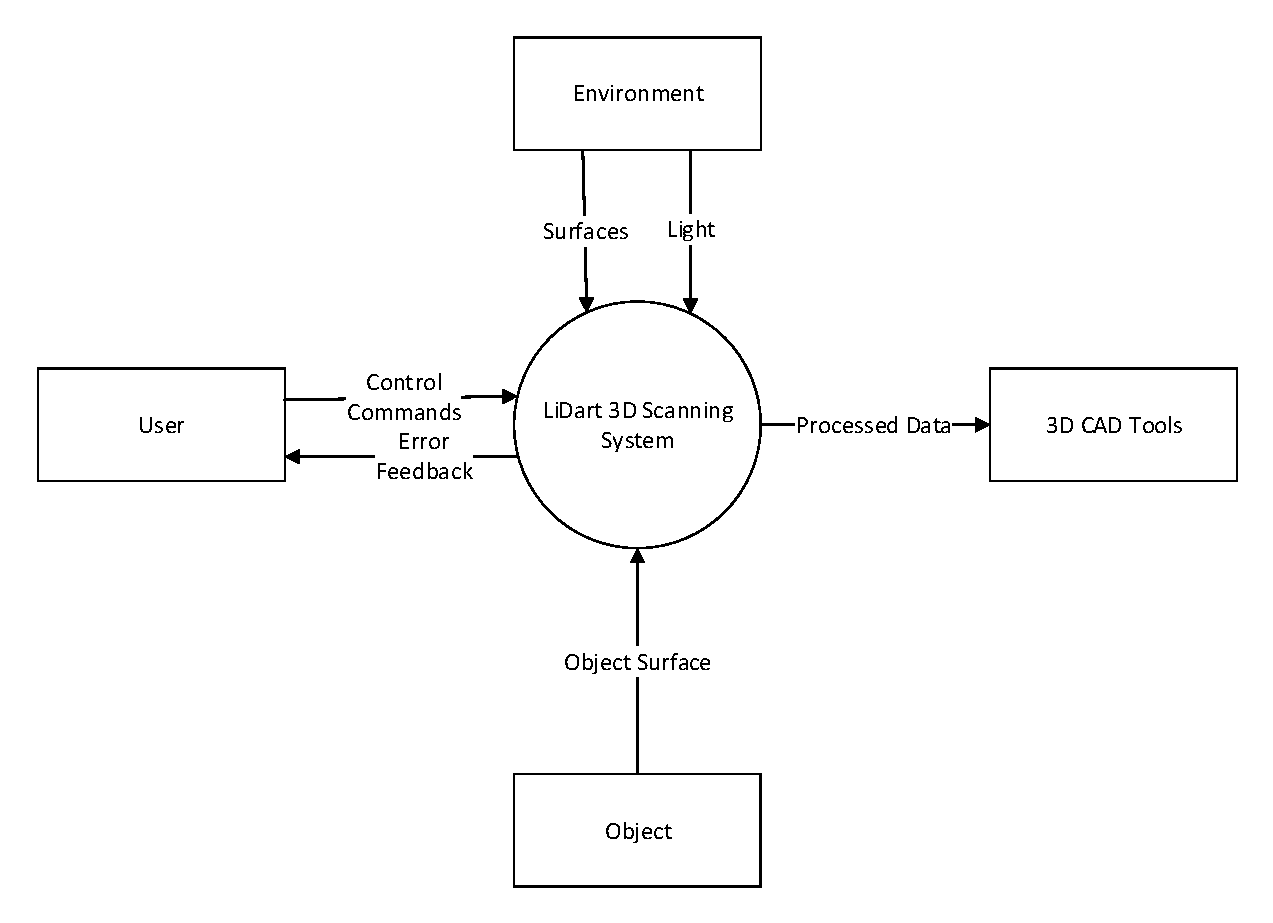
\includegraphics[width=1\textwidth]{Figures/Context Diagram.pdf}
\caption{System Context Diagram}
\label{Fig_SystemContext} 
\end{center}
\end{figure}

\section{Project Overview}
\label{sec_ProjOverview}

\subsection{Normal Behaviour}

\progname~ is a remote-controlled robot that is operated by a user through a web-based user interface. In order to obtain scans, location markers must be set up in the environment surrounding the robot. The user will drive the robot to the desired scanning location by specifying the direction of movement on the user interface. Live camera feed will be displayed on the user interface to aid with navigation. Once the robot is at the desired location, the user can direct the robot to begin scanning through the user interface. The robot will continuously perform state estimation while taking scans through the LiDAR sensor. After scanning is complete, the point-cloud data will be stitched together to create the final 3D scan, which can then be saved as a .obj file. \\

\noindent Normal operation of the LiDart system will proceed as follows:
\begin{enumerate}
\item Robot is powered on
\item User connects to the robot via WiFi
\item User opens the GUI
\item User drives the robot to a desired location, the user can use the live video feed and LiDAR data preview to choose such a location
\item User initiates a scan
\item Steps 4 and 5 are repeated until the user has scanned all desired areas of the environment
\item User downloads the final stitched 3D scan    
\end{enumerate}

\subsection{Undesired Event Handling}

\wss{How you will approach undesired events}

\progname~ will detect error conditions due to undesired events and alert the user of any errors. Messages shall be displayed on the user interface to alert the user of errors and suggest steps to correct these errors. In a situation where the error cannot be resolved, the robot will need to be manually reset. Several events that fall outside of normal operations are described in the following sections.

\subsubsection{\textbf{Cancelling a Scan}} If the user has initiated a scan but then decides that the location is not ideal, the user can cancel the scan. This discards the information from that specific scan and allows the user to resume driving the robot.

\subsubsection{\textbf{Robot Not Localized}} If the robot is not localized, it will not allow the user to initiate a scan. To be able to initiate a scan the user must first drive the robot to a location where the robot can localize itself.

\subsubsection{\textbf{Emergency Stopping}} If the robot begins misbehaving it can be powered off with an onboard emergency stop switch. This is required in the event that a hardware failure causes the robot to pose a safety risk or to stop responding to user commands.

\subsection{Component Diagram}

Figure~\ref{Fig_FunctionalDecomposition} depicts the decomposition of \progname~ into sub-systems. \progname consists of a user interface, an on-board computing module, robot inputs (sensors), and robot outputs (actuators). The embedded software running on the robot is further subdivided into modules which are described in detail in the Module Interface Specification and Module Guide documents.
 
\begin{figure}[H]
\begin{center}
    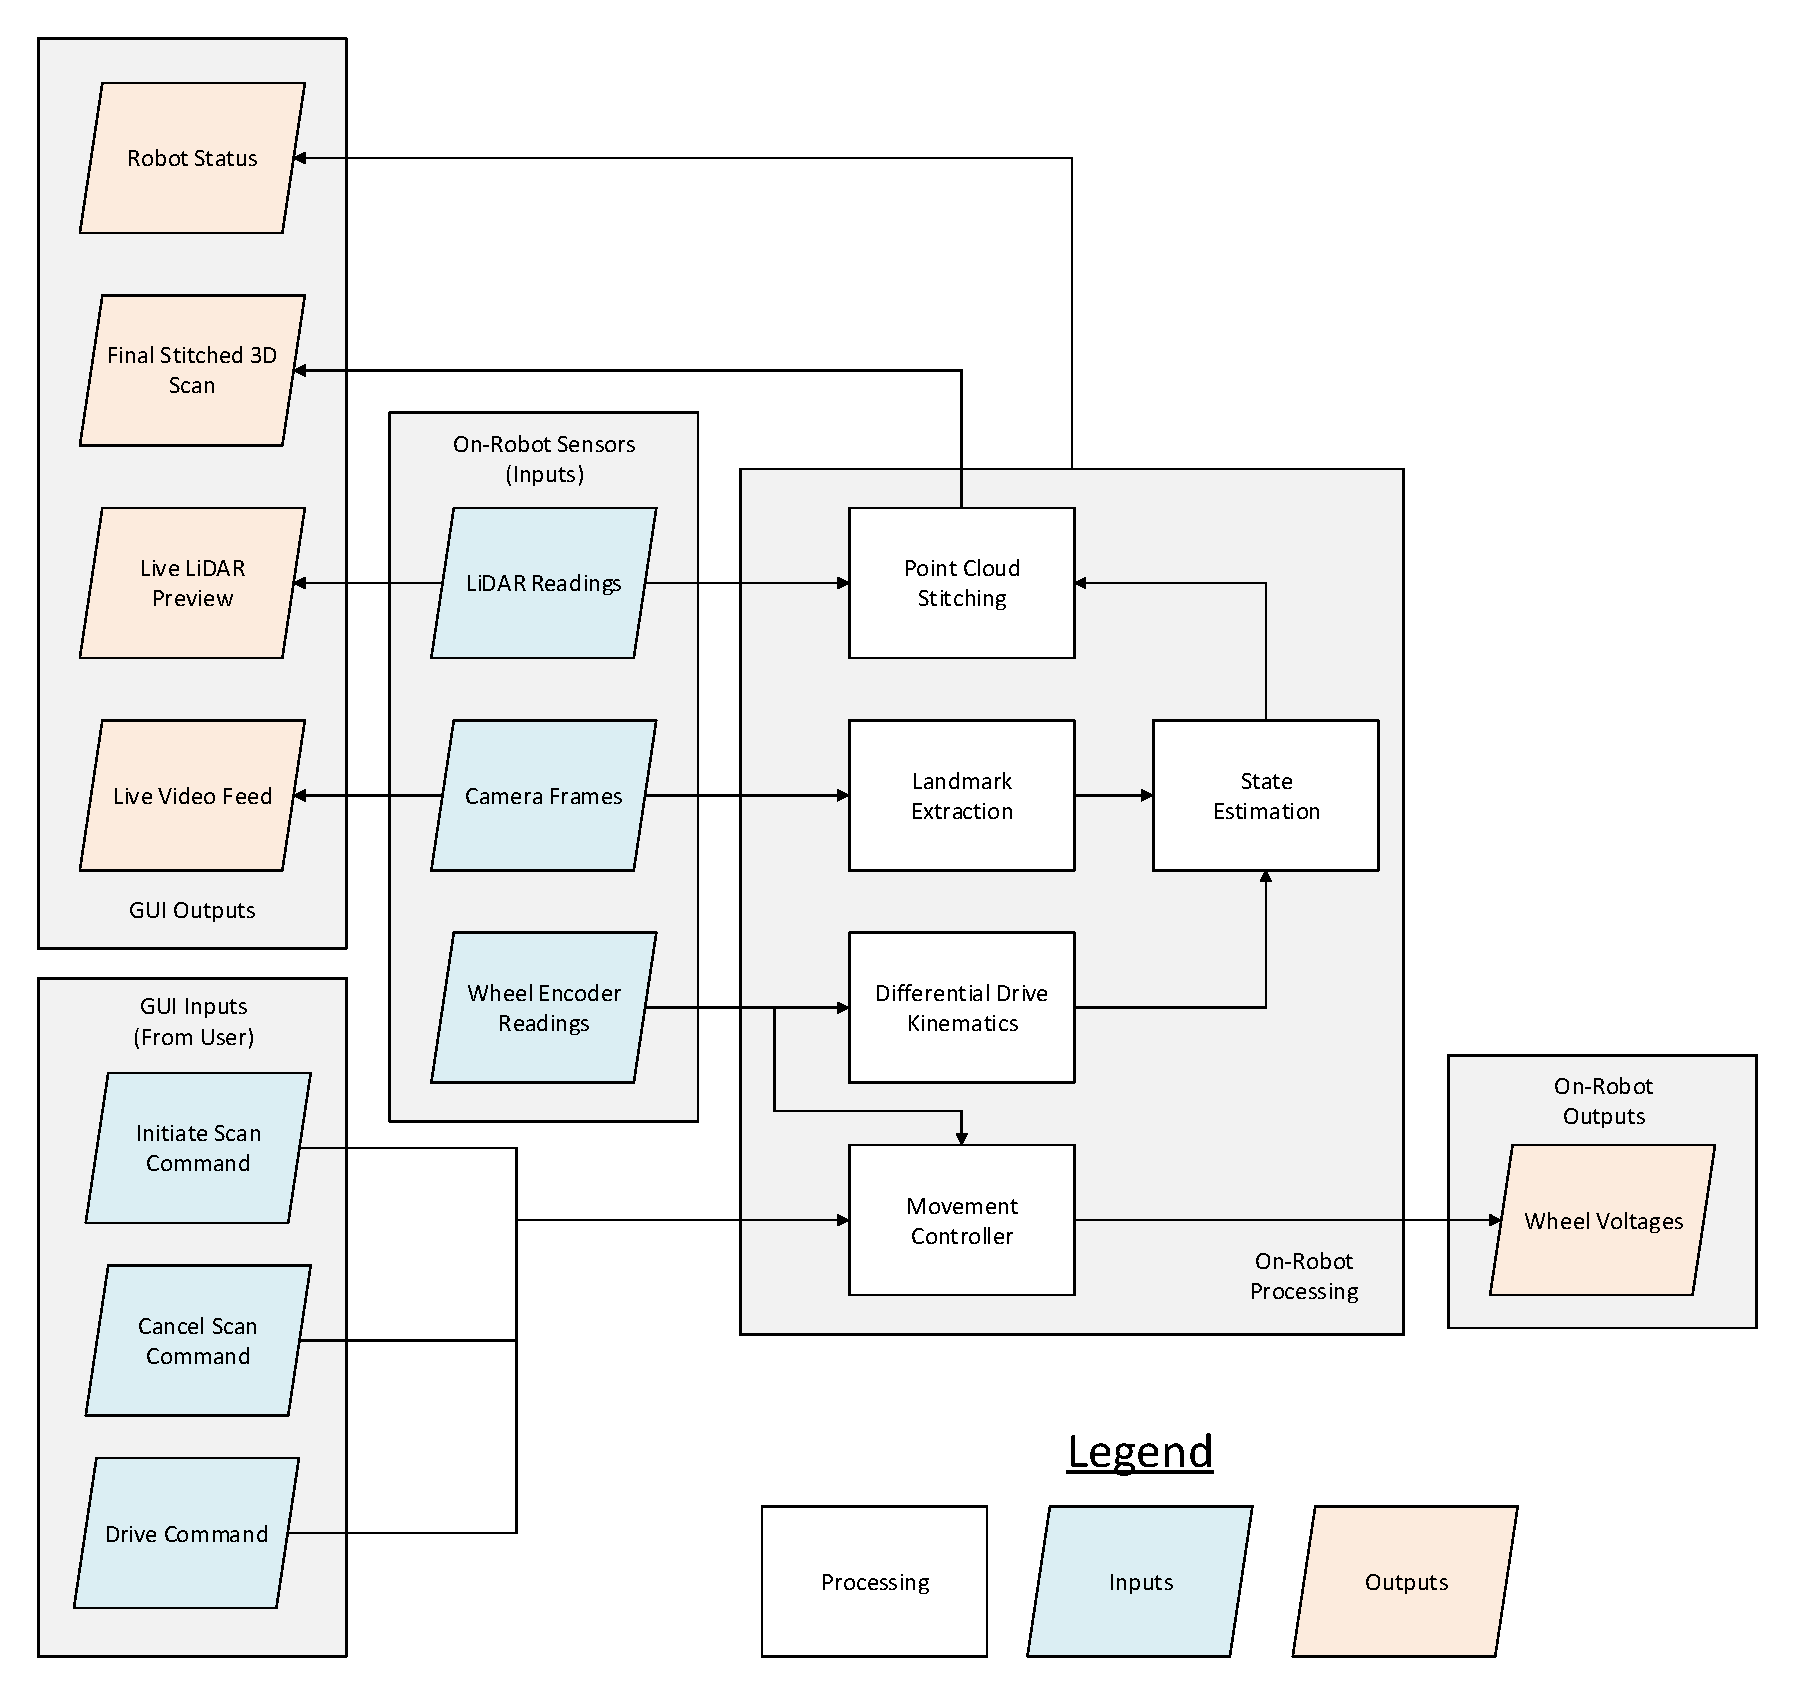
\includegraphics[width=0.85\textwidth]{Figures/Functional Decomposition.pdf}
\caption{Functional Decomposition Diagram}
\label{Fig_FunctionalDecomposition} 
\end{center}
\end{figure}

\subsection{Connection Between Requirements and Design} \label{sec_Connection}

\wss{The intention of this section is to document decisions that are made
  ``between'' the requirements and the design.  To satisfy some requirements,
  design decisions need to be made.  Rather than make these decisions implicit,
  they are explicitly recorded here.  For instance, if a program has security
  requirements, a specific design decision may be made to satisfy those
  requirements with a password.}
  
Table~\ref{Table:Traceability} shows the traceability between design components and requirements specified in the SRS.
  
\begin{table}[H]
\caption{Traceability between system components and requirements}
\label{Table:Traceability}
\begin{tabularx}{\textwidth}{|l|X|}
\hline
\textbf{Component}       & \textbf{Requirement} \\ \hline
User Interface Inputs    &                      \\ \hline
User Interface Outputs   &                      \\ \hline
On-Board Robot Inputs    &                      \\ \hline
On-Board Robot Actuators &                      \\ \hline
\end{tabularx}
\end{table}

\section{System Variables}
\label{sec_SysVars}

\wss{Include this section for Mechatronics projects}

This section defines the monitored, controlled, and constant system variables.

\subsection{Monitored Variables}

Table~\ref{Table:m_var} specifies the variables that are measured by the system.

\begin{table}[H]
\caption{Monitored Variables}
\label{Table:m_var}
\begin{tabularx}{\textwidth}{|l|l|c|c|X|}
\hline{\bf Name} & {\bf Type} & \multicolumn{1}{l|}{\bf Range} & \multicolumn{1}{l|}{\bf Units}& {\bf Description}\\
\hline
 m\_InitScan & boolean & [0,1] & - & Initiate scan command\\
\hline
 m\_CancelScan & boolean & [0,1] & - & Cancel scan command\\
\hline
m\_Forward & boolean & [0,1] & - & Move robot forwards command\\
\hline
m\_Backward & boolean & [0,1] & - & Move robot backwards command\\
\hline
m\_Right & boolean & [0,1] & - & Move robot to the right command\\
\hline
m\_Left & boolean & [0,1] & - & Move robot to the left command\\
\hline
m\_ExportScan & boolean & [0,1] & - & Export scan command\\
\hline
m\_Battery & float &  &  & Battery level reading\\
\hline
m\_Distance & float & [200-12000] & mm & Distance between the rotating core of the LiDAR sensor and the sampling point\\
\hline
m\_Heading & float & [0-360] & deg & Angle of the LiDAR sensor measurement\\
\hline
m\_StartFlag & boolean & [0,1] & n/a & Flag to start a new LiDAR scan\\
\hline
m\_Checksum & int &  & n/a & Checksum of the LiDAR data\\
\hline
\end{tabularx}
\label{Table:m_var}
\end{table}

\subsection{Controlled Variables}

Table~\ref{Table:c_var} specifies the variables that are controlled by the system.

\begin{table}[H]
\caption{Controlled Variables}
\label{Table:c_var}
\begin{tabularx}{\textwidth}{|l|l|c|c|X|}
\hline{\bf Name} & {\bf Type} & \multicolumn{1}{l|}{\bf Range} & \multicolumn{1}{l|}{\bf Units}& {\bf Description}\\
\hline
o\_WheelRight & int & [0-5] & V & Right wheel output voltage \\
\hline
o\_WheelLeft & int & [0-5] & V & Left wheel output voltage \\
\hline
o\_Staus & int & [0-4] & n/a & Robot state (fault, idle, waiting for connection, ready to scan, scanning) \\
\hline
o\_ErrorState & string & n/a & n/a & State estimation error message\\ \hline
o\_ErrorObstacle & string & n/a & n/a & Obstacle error message\\ \hline
o\_ErrorWifi & string & n/a & n/a & WiFi connection error message\\ \hline
o\_ErrorBattery & string & n/a & n/a & Low battery level error message\\ \hline
o\_ScanOut & .obj file & n/a & n/a & file containing 3D scan\\ \hline
o\_Camera & binary & n/a & n/a & Live video feed\\ \hline
\end{tabularx}
\label{Table:c_var}
\end{table}

\subsection{Constants Variables}

Table~\ref{Table:constants} specifies the system constants.

\begin{table}[H]
\caption{Constants}
\label{Table:constants}
\begin{tabularx}{\textwidth}{|l|l|c|c|X|}
\hline{\bf Name} & {\bf Type} & \multicolumn{1}{l|}{\bf Range} & \multicolumn{1}{l|}{\bf Units}& {\bf Description}\\
\hline
 &  &  &  & \\
\hline
 &  &  &  & \\
\hline
 &  &  &  & \\
\hline
 &  &  &  & \\
\hline
\end{tabularx}
\label{Table:constants}
\end{table}

- state estimation?, movement controller physical quantities i.e. wheel voltages, physical dimensions/properties of the robot, communication protocol constants i.e. baude rate

\section{User Interfaces}
\label{sec_User}

\wss{Design of user interface for software and hardware.  Attach an appendix if
needed. Drawings, Sketches, Figma}

The user interface is accessible using a smart device with WiFi capability. The user interface is used to control the movement of the robot, instruct the robot to start scanning, and save the data on the user's device. The main area of the user interface is used to display live video feed from web-cams attached to the robot. A horizontal bar across the top of the interface provides buttons to control the robot, start/stop scanning operations, and save the scanning data. The keyboard arrow keys may also be used to move the robot. Sketches of the user interface are provided in Appendix~\ref{Interface}.


\section{Design of Hardware}
\label{sec_Mech}

\wss{Most relevant for mechatronics projects}
\wss{Show what will be acquired}
\wss{Show what will be built, with detail on fabrication and materials}
\wss{Include appendices as appropriate, possibly with sketches, drawings, CAD, etc}

- aluminum frame chassis\\
- omni-directional wheels (holonomic robot design)\\
- mounts for cameras, LiDAR sensor\\
- enclosure for electronics\\

CAD renderings of the robot are provided in Appendix~\ref{Mechanical_Hardware}.

\section{Design of Electrical Components}
\label{sec_Elec}

\wss{Most relevant for mechatronics projects}
\wss{Show what will be acquired}
\wss{Show what will be built, with detail on fabrication and materials}
\wss{Include appendices as appropriate, possibly with sketches, drawings,
circuit diagrams, etc}

LiDart uses a micro-processor based embedded system to run the GUI and control the robot. A Raspberry Pi hosts a web-server for the GUI, interfaces with peripheral devices, and processes data obtained from the LiDAR sensor. The Raspberry Pi communicates with peripheral devices over USB), including cameras, the LiDAR sensor, and an Arduino micro-controller. The Arduino is used to drive a dual H-bridge motor driver which controls two DC motors. A circuit diagram and bill of materials is provided in Appendix~\ref{Electrical_Components}.

\section{Design of Communication Protocols}
\label{sec_Comm}

\wss{If appropriate}

USB (Universal Serial Bus) is used to communicate between the Raspberry Pi controller and peripheral devices. WiFi is used to communicate between the user's smart device, such as a cellphone or laptop, and the robot.

\section{Timeline}
\label{sec_Timeline}

\wss{Schedule of tasks and who is responsible}

Table~\ref{Table:Timeline} defines the design tasks and team member responsibilities. 

\begin{table}[H]
\caption{Design Timeline}
\label{Table:Timeline}
\begin{tabularx}{\textwidth}{|X|p{0.2\textwidth}|p{0.31\textwidth}|}
\hline
\textbf{Task}                                    & \textbf{Team Member} & \textbf{Date}             \\ \hline
Rev 0 mechanical design, procurement/fabrication of components, and mechanical assembly & Neeraj Ahluwalia & 09/Jan/2023 - 23/Jan/2022 \\ \hline
Rev 0 electrical design, procurement of components, and electrical assembly   \newline Modules: Movement controller  & Michaela Schnull & 09/Jan/2023 - 23/Jan/2022 \\ \hline
Rev 0 development of the frontend/user interface \newline Modules: Frontend & Karim Elmokattaf     & 09/Jan/2023 - 23/Jan/2022 \\ \hline
Rev 0 development of the state estimation/point-cloud stitching software \newline Modules: State estimation, point-cloud stitching, landmark extraction, differential drive kinematics & Jonathan Casella & 09/Jan/2023 - 23/Jan/2022 \\ \hline
Rev 0 integration testing                        & All                  & 24/Jan/2023 - 06/Feb/2022 \\ \hline
\end{tabularx}
\end{table}

\newpage
\bibliographystyle{ieeetr}
\bibliography{references}

\newpage{}

\appendix

\section{Interface}
\label{Interface}

\wss{Include additional information related to the appearance of, and
interaction with, the user interface}

\section{Mechanical Hardware}
\label{Mechanical_Hardware}
Insert CAD assembly diagram and BOM here.\\


\begin{landscape}
\section{Electrical Components}
\label{Electrical_Components}

\vspace*{\fill}
\begin{figure}[H]
\begin{center}
 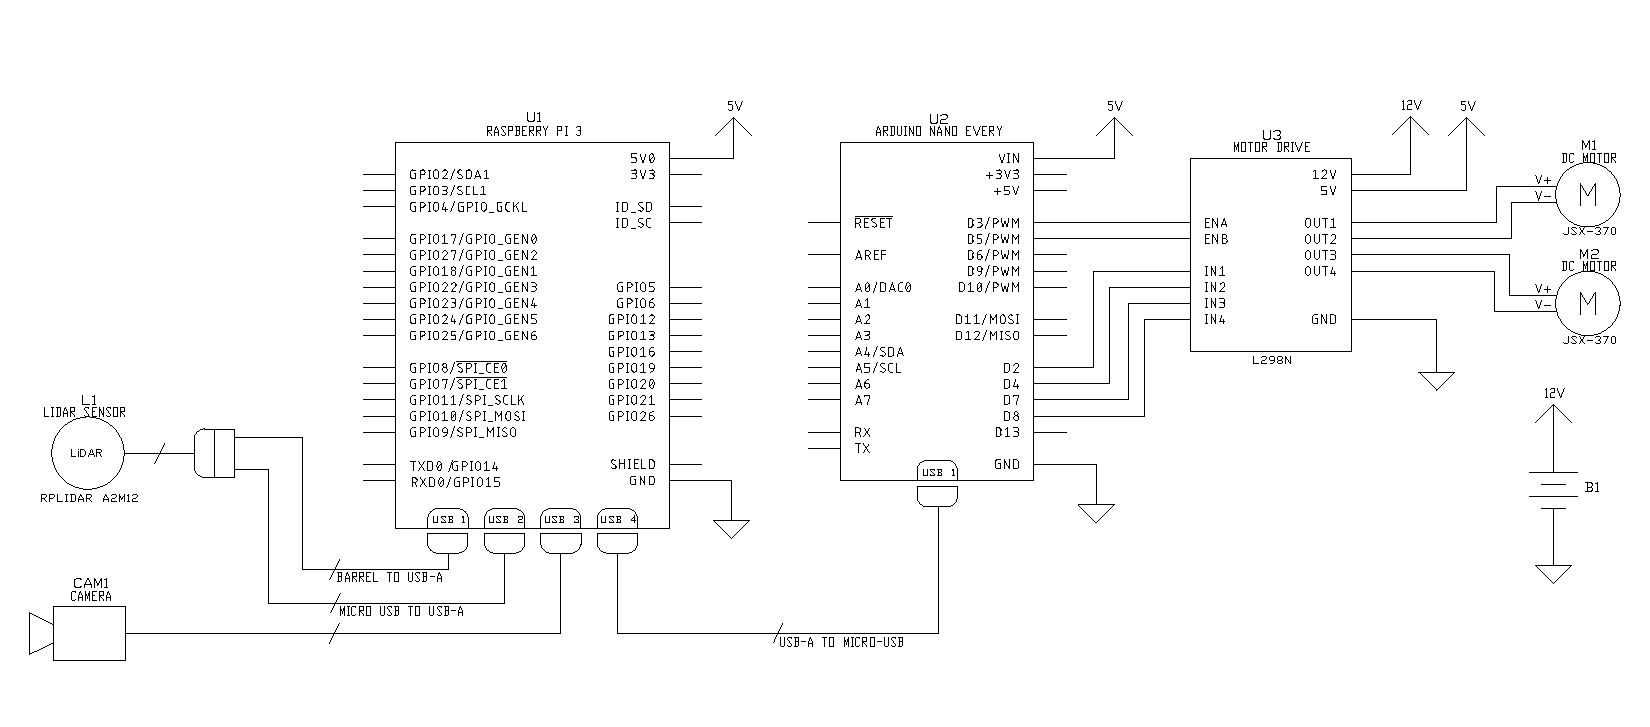
\includegraphics[width=1.25\textwidth]{Figures/Circuit Diagram.pdf}
\caption{Circuit Diagram}
\label{Fig_CircuitDiagram} 
\end{center}
\end{figure}
\vspace*{\fill}
\end{landscape}

\begin{table}[H]
\caption{Bill of Materials - Electrical}
\label{Table:bom-elec}
\resizebox{\textwidth}{!}{%
\begin{tabular}{|l|l|c|l|}
\hline
\textbf{Part Number} & \textbf{Description} & \multicolumn{1}{l|}{\textbf{Quantity}} & \textbf{Reference Designator} \\ \hline
Slamtec RPLIDAR A2M12 & 360-degree 2D laser scanner (LiDAR)  & 1 & L1               \\ \hline
Raspberry Pi Rev 3    & Single board computer                & 1 & U1               \\ \hline
Arduino Nano Every    & ATMega4809 AVR microcontroller board & 1 & U2               \\ \hline
L298N                 & Dual H-Bridge Driver IC Board        & 1 & U3               \\ \hline
JSX-370               & DC 12V Gear Reduction Motor          & 2 & M1, M2           \\ \hline
TBD                   & Mini-Webcam USB                      & 1 & CAM1 \\ \hline
12V DC Battery        & 12V DC Battery                       & 1 & B1               \\ \hline
TBD        		  	  & Switch 
& 1 & SW1               \\ \hline
\end{tabular}%
}
\end{table}

\section{Communication Protocols}

\section{Reflection}

The information in this section will be used to evaluate the team members on the
graduate attribute of Problem Analysis and Design.  Please answer the following questions:

\begin{enumerate}
  \item What are the limitations of your solution?  Put another way, given
  unlimited resources, what could you do to make the project better? (LO\_ProbSolutions)
  
\subsection{Cost Limitations}
Cost constraints imposed limitations on the \progname~ solution. An inexpensive LiDAR sensor with reduced accuracy and range compared to more expensive solutions was used due to the limited budget. The more expensive LiDAR sensor would improve the accuracy of data obtained and enable larger areas to be scanned. Limited funding also limited the mechanical design of the robot. The robot used primarily 3D printed components. Custom machined components are more expensive, however wold improve the durability, reliability, and tolerances of the robot. A custom PCB (printed circuit board) could also be designed instead of various connected boards This would reduce number of components and improve the reliability and maintainability of the system.
  
\subsection{Localization Accuracy}
Additional sensors could be added to improve the localization of the robot, such as wheel encoders and accelerometers. Sensor fusion could be implemented to improve the state estimation algorithms, resulting in and increase in the accuracy of scans.
  
\subsection{Autonomous Scanning}
The operation of the robot in the specified design requires the user to remotely pilot the robot. Since this could be time consuming for the user, an additional feature that LiDart could implement is autonomous scanning. While autonomously scanning, the robot would explore its environment without any user intervention. Implementing autonomous scanning would require the development of additional software.\\
  
  \item Give a brief overview of other design solutions you considered.  What
  are the benefits and tradeoffs of those other designs compared with the chosen
  design?  From all the potential options, why did you select documented design?
  (LO\_Explores)
  
\subsection{User Interface}
A desktop graphical user interface and web-based user interface were considered. The web based user interface was selected due to its flexibility, portability, and ease-of-use. A user can simply connect to the web-hosted interface instead of having to install a desktop application. A disadvantage of the web-hosted user interface is limited functionality compared to a desktop application.
  
\subsection{Holonomic Robot Design}
Holonomic and non-holonomic robot designs were considered. A holonomic robot design was chosen due to greater maneuverability and ability to navigate through small and narrow spaced. A drawback of using holonomic robots was that omni-directional wheels must be used which are not standard and have less traction.
  
\subsection{Localization Markers}
Round spherical markers and April Tags \cite{olson2011tags} were considered as markers used for the robot state estimation. April Tags provided many advantages compared to the round coloured markers. Unlike generic round markers, April Tags do not need to be calibrated, which is a time consuming and error-prone process. They are also easier to detect, and provide additional information such as the angle, resulting in more accurate state estimation.\\
  
  
\end{enumerate}

\end{document}